% (The MIT License)
%
% Copyright (c) 2023-2024 Yegor Bugayenko
%
% Permission is hereby granted, free of charge, to any person obtaining a copy
% of this software and associated documentation files (the 'Software'), to deal
% in the Software without restriction, including without limitation the rights
% to use, copy, modify, merge, publish, distribute, sublicense, and/or sell
% copies of the Software, and to permit persons to whom the Software is
% furnished to do so, subject to the following conditions:
%
% The above copyright notice and this permission notice shall be included in all
% copies or substantial portions of the Software.
%
% THE SOFTWARE IS PROVIDED 'AS IS', WITHOUT WARRANTY OF ANY KIND, EXPRESS OR
% IMPLIED, INCLUDING BUT NOT LIMITED TO THE WARRANTIES OF MERCHANTABILITY,
% FITNESS FOR A PARTICULAR PURPOSE AND NONINFRINGEMENT. IN NO EVENT SHALL THE
% AUTHORS OR COPYRIGHT HOLDERS BE LIABLE FOR ANY CLAIM, DAMAGES OR OTHER
% LIABILITY, WHETHER IN AN ACTION OF CONTRACT, TORT OR OTHERWISE, ARISING FROM,
% OUT OF OR IN CONNECTION WITH THE SOFTWARE OR THE USE OR OTHER DEALINGS IN THE
% SOFTWARE.

\documentclass{article}
\usepackage{../osbp}
\newcommand*\thetitle{Setting Guidelines}
\begin{document}

\plush{\osbpTitlePage{5}{mWi2S5FJiJ4}}

\thought{Have \ff{LICENSE.txt} file with an MIT license in your repository}

\qte
  [Arnoud Engelfriet]
  {arnoud-engelfriet}
  {Perhaps the \ul{most difficult} issue when setting up the project is which license to choose... No one will contribute code just because it's GPL or BSD. But with the \ul{wrong license}, your chances of a successful open source release are slim.}
  {engelfriet2009choosing}

\qte
  [Richard Stallman]
  {richard-stallman}
  {\textbf{copyleft}: Everyone will be permitted to modify and redistribute GNU, but no distributor will be allowed to restrict its further redistribution. That is to say, \ul{proprietary} modifications will \ul{not be allowed}. I want to make sure that all versions of GNU remain free.}
  {stallman1985gnu}

\plush{\pptBanner{Which license to choose?}
  \begin{tabular}{lll}
  \toprule
  License & Type \\
  \midrule
  Massachusetts Institute of Technology (\textbf{MIT}) & Copyright \\
  \textbf{Apache} & Copyright \\
  Berkeley Software Distribution (\textbf{BSD}) & Copyright \\
  GNU Public License (\textbf{GPL}) & Copyleft \\
  \bottomrule
  \end{tabular}}

\plush{\pptBanner{What permissions may be granted by a license?}
  \begin{itemize}\setlength\itemsep{0em}
  \item Permission to \ul{use}
  \item Permission to \ul{modify}
  \item Permission to \ul{distribute}
  \item Permission to \ul{not mention} the product
  \item Permission to \ul{remove copyright notice}
  \end{itemize}
  \source{lin2006open}}
\pitch{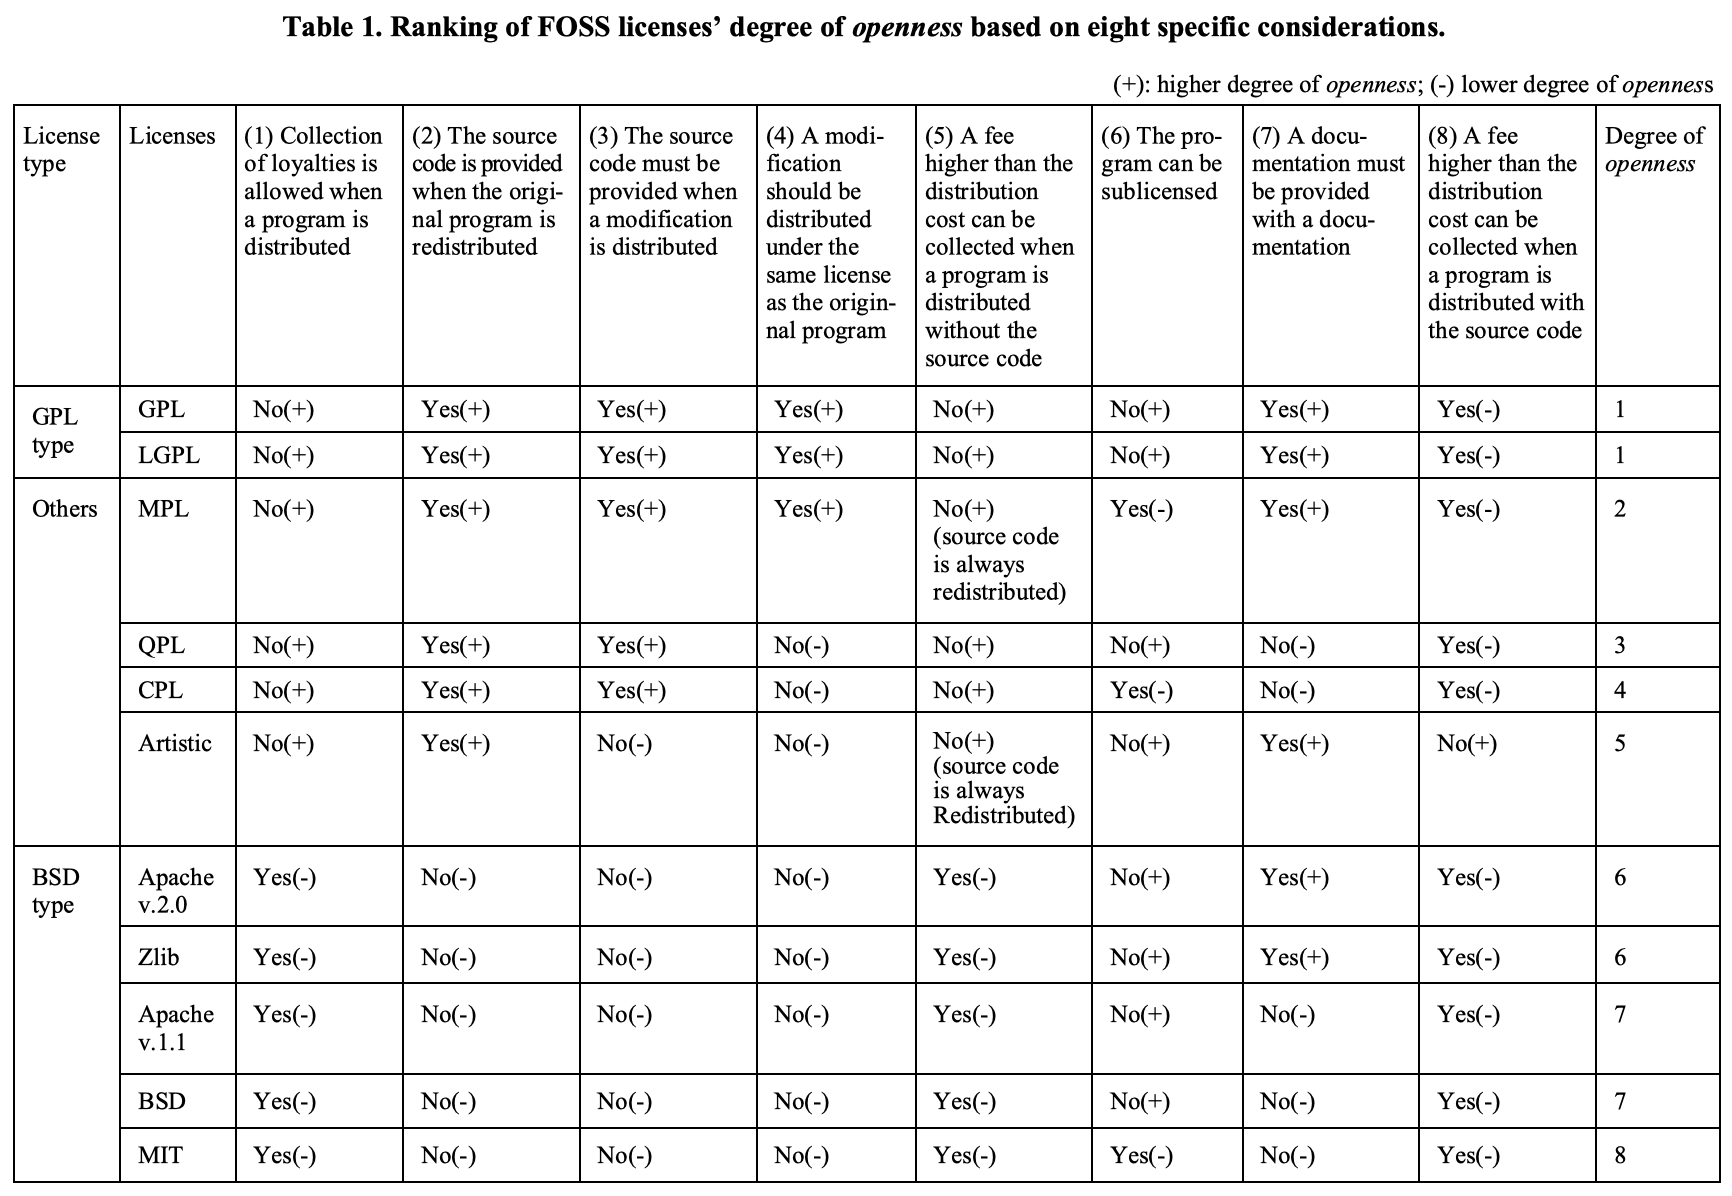
\includegraphics[width=.6\linewidth]{openness.png}
  \source{lin2006open}}

\qte
  [Ben Balter]
  {ben-balter}
  {Unsurprisingly, \ul{MIT}, \ul{Apache}, and \ul{GPL} are the clear front runners, with some 15\% of licensed projects opting for a non-standard license.}
  {github2015licenses}
\pitch{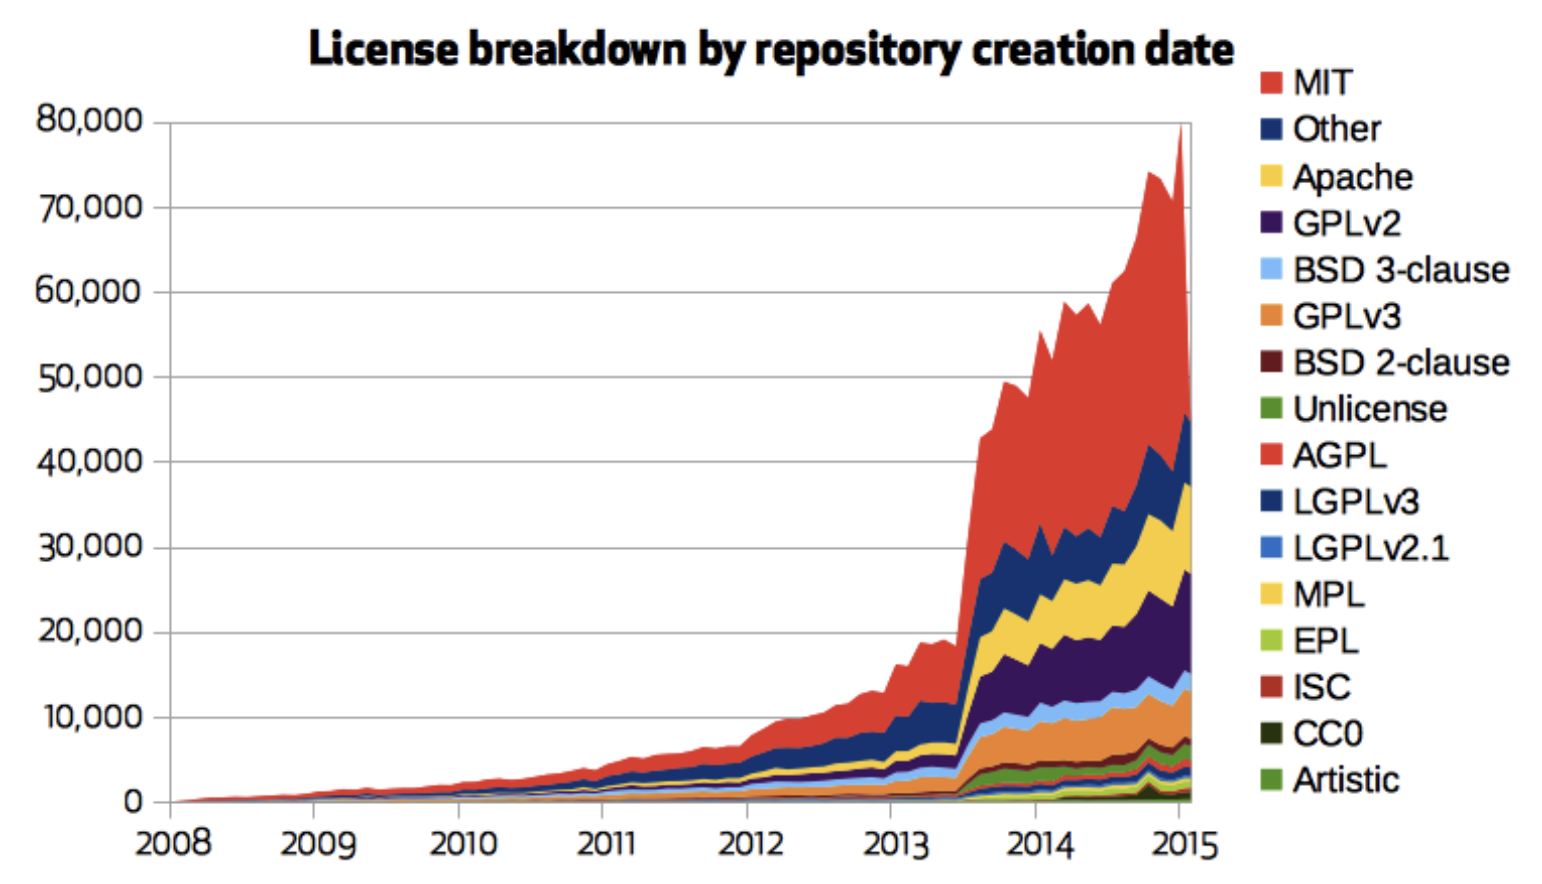
\includegraphics[width=.7\linewidth]{licenses.png}
  \source{github2015licenses}}

\thought[bugayenko2019blog0423]{Make the \ff{README.md} file attractive}

\plush{\pptBanner{Mandatory sections of \ff{README.md}:}
  \begin{itemize}\setlength\itemsep{0em}
  \item Title, logo, badges
  \item What is it? What problem does it solve?
  \item How to quick start?
  \item How to contribute?
  \item Who is who?
  \end{itemize}
  \source{bugayenko2019blog0423}}

\qte
  [Gede Artha Azriadi Prana]
  {gede-prana}
  {We conduct a qualitative study involving the manual annotation of 4,226 README file sections from 393 randomly sampled GitHub repositories. We find that information discussing the `What' and `How' of a repository is very common, while many README files lack information regarding the \ul{purpose} and \ul{status} of a repository.}
  {prana2019categorizing}

\qte
  [Simon Weber]
  {simon-weber}
  {Upon investigation, popular projects were found to have larger READMEs (median 2 kilobytes vs. 500 bytes). Also, 95\% of popular projects have nonempty READMEs, compared to only 65\% of unpopular projects.}
  {weber2014makes}
\pitch{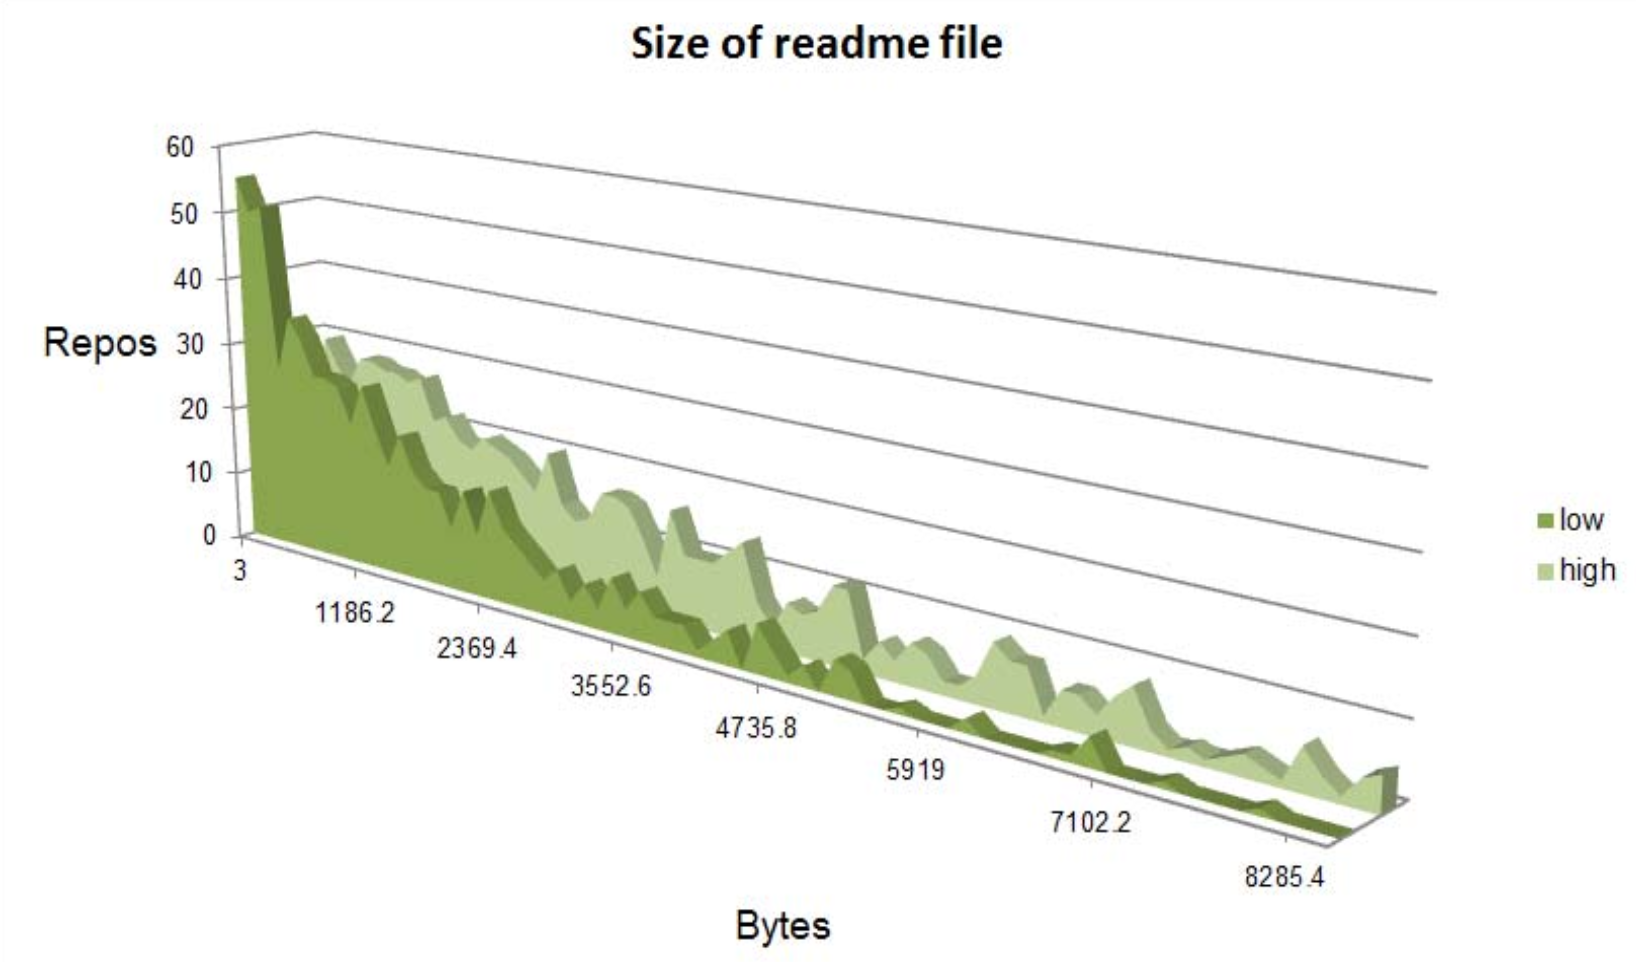
\includegraphics[width=.75\linewidth]{readme-size.png}
  \source{weber2014makes}}

\qte
  [\nospell{Asher Trockman}]
  {asher-trockman}
  {We find that non-trivial \ul{badges}, which display the build status, test coverage, and up-to-dateness of dependencies, are mostly reliable signals, correlating with more tests, better pull requests, and fresher dependencies.}
  {trockman2018adding}

\thought[bugayenko2014blog0721]{Make the \ff{master} branch read-only}

\thought{Put \ff{CODE\_OF\_CONDUCT.md} file to your repository... not}

\qte
  [Parastou Tourani]
  {parastou-tourani}
  {We found that the top codes of conduct are adopted by hundreds to thousands of projects, while all of them share five common dimensions.}
  {tourani2017code}
\pitch{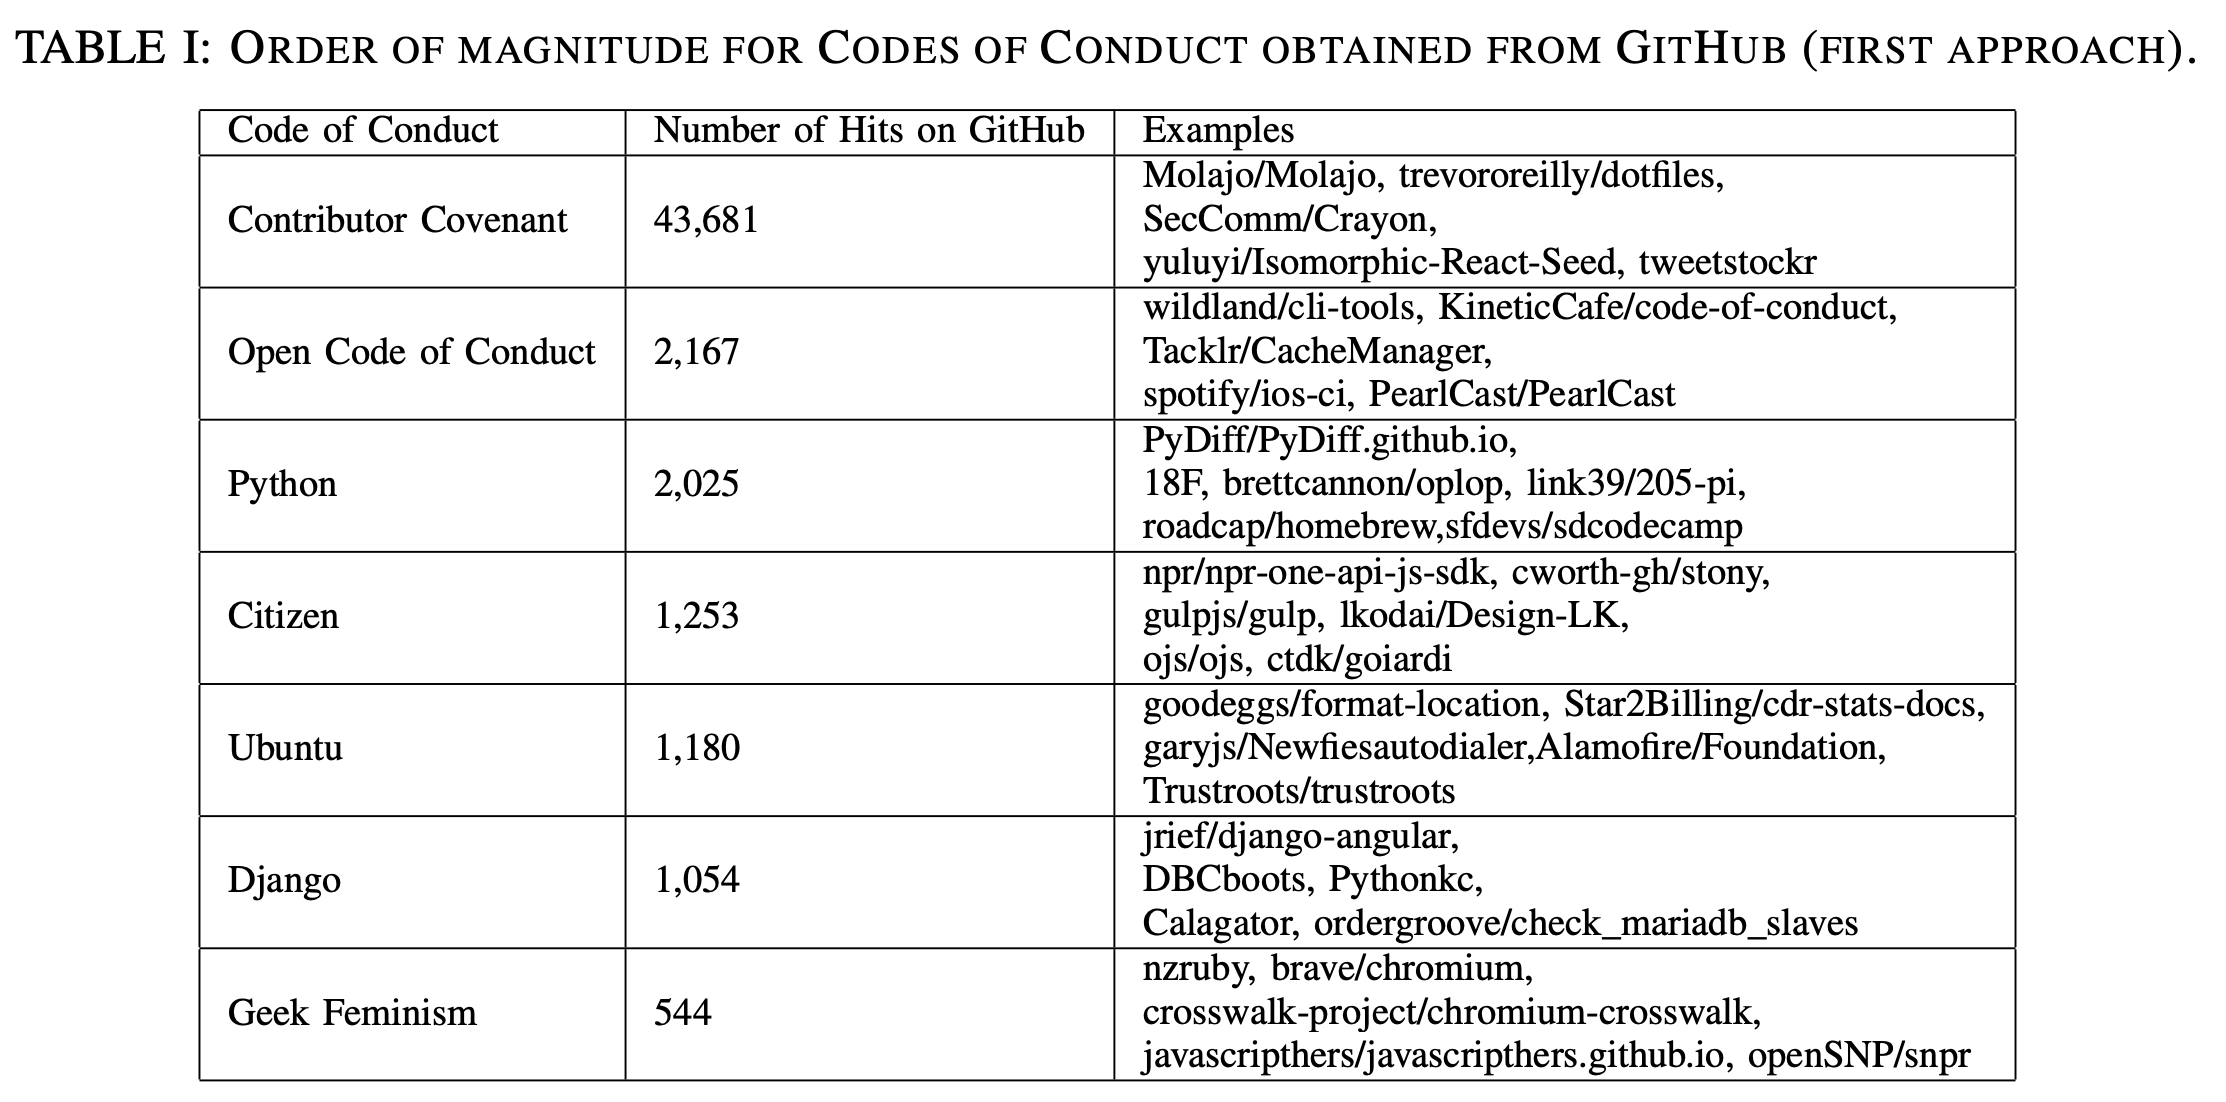
\includegraphics[width=.8\linewidth]{codes.png}
  \source{tourani2017code}}
\pitch{
  \begin{multicols}{2}
  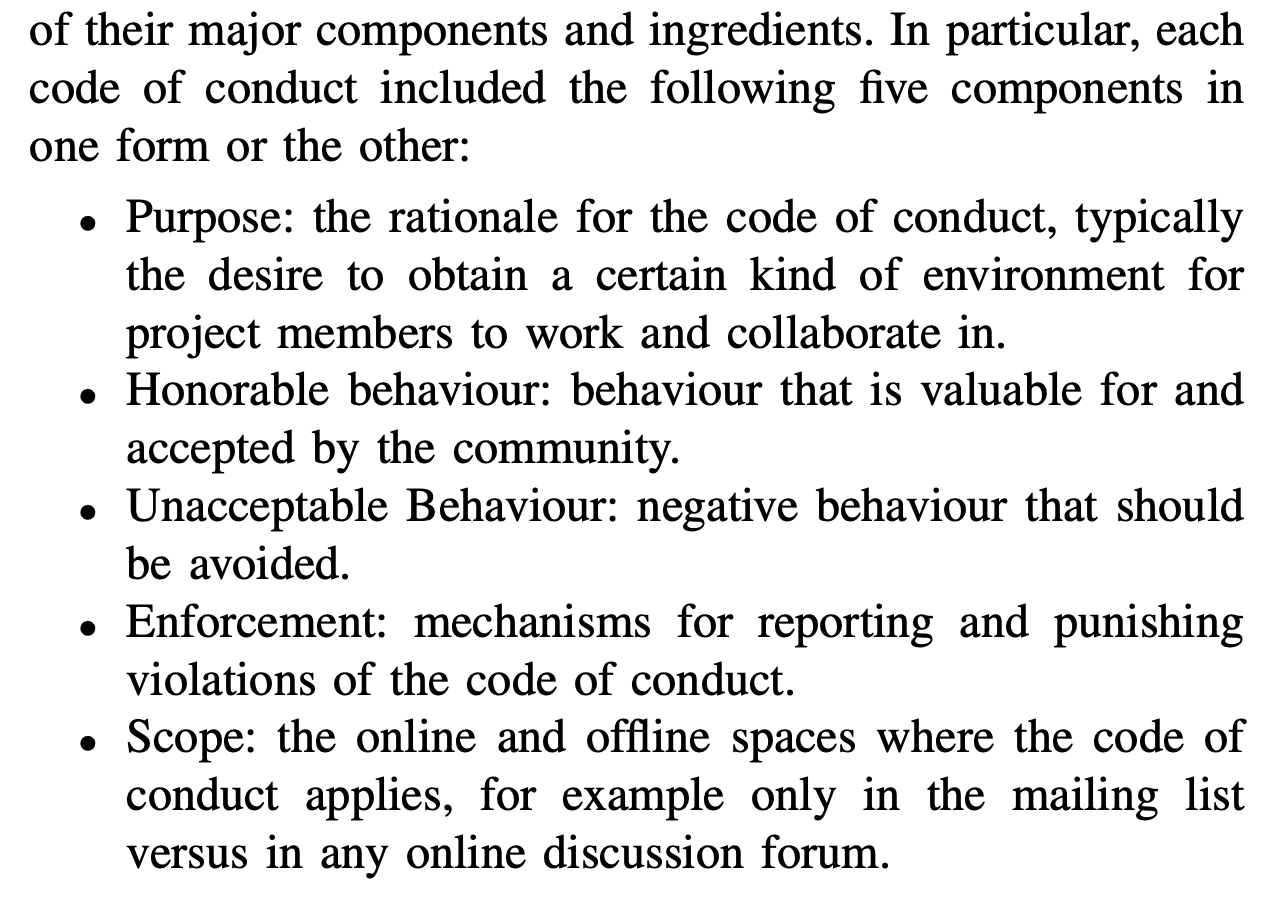
\includegraphics[width=.9\linewidth]{dimensions.png}
  \source{tourani2017code}
  \par\columnbreak\par
  ``The Contributor Covenant explicitly mentions sexualized language or imagery, trolling, insulting and publishing of private information of others as unexpected behaviors. Django adds discriminatory jokes and violent threats to this list. Geek Feminism and the Open code of conduct provide a more detailed list, ...''
  \end{multicols}}

\plush{\pptBanner{Django Code of Conduct}
  ``We strive to be a community that welcomes and supports people of \ul{all} backgrounds and identities. This includes, but is not limited to members of any race, ethnicity, culture, national origin, colour, immigration status, social and economic class, educational level, sex, sexual orientation, gender identity and expression, age, size, family status, \ul{political belief}, religion, and mental and physical ability.''}

\qte
  [Hana Frluckaj]
  {hana-frluckaj}
  {Even though including a code of conduct is considered a \ul{best practice} recommendation to \ul{attract} newcomers, there is, as of yet, no \ul{empirical} evidence backing up that claim.}
  {li2021code}

\qte
  [Dabbish Laura]
  {dabbish-laura}
  {We found that projects in our sample \ul{did not} extensively discuss the addition or changes to the code of conduct.}
  {li2021code}

\qte
  [Jack Jamieson]
  {jack-jamieson}
  {We found multiple significant relationships between value-related discussions and turnover, including that discussions about \ul{respectfulness} predict an increase in contributors leaving and a decrease in new contributors, while discussions about \ul{social power} predicted better contributor retention.}
  {jamieson2023predicting}

\thought{Don't explain coding guidelines, setup GitHub Action checks}

\qte
  [Timothy Kinsman]
  {timothy-kinsman}
  {We analyzed the effect of adoption across 926 projects that had adopted GitHub Actions for at least 6 months. Our findings indicate that, on average, there are \ul{more rejected pull requests} and fewer commits on merged pull requests after adopting GitHub Actions.}
  {kinsman2021software}

\qte
  [Alexandre Decan]
  {alexandre-decan}
  {We observed that workflows tend to be used in the \ul{more active} GitHub projects (more contributors, pull requests, commits and issues).}
  {decan2022use}
\pitch{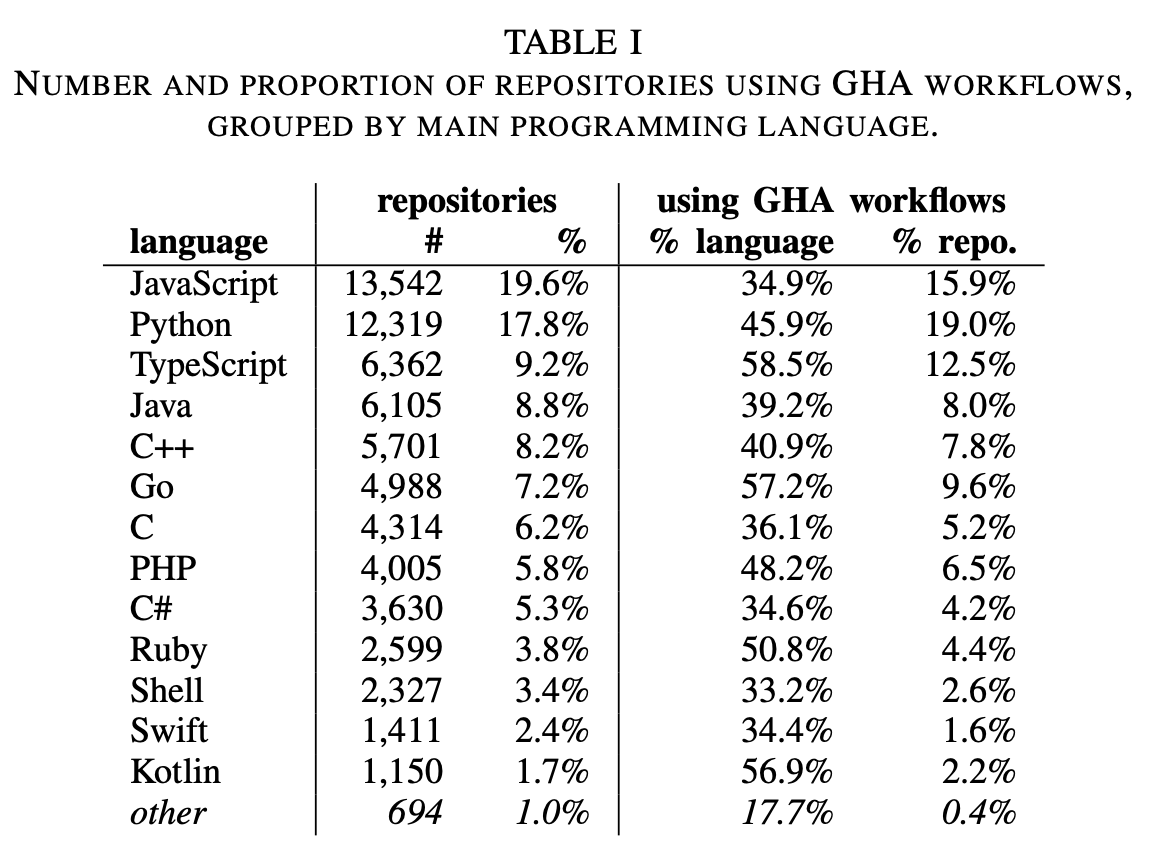
\includegraphics[width=.6\linewidth]{by-language.png}
  \source{decan2022use}}
\pitch{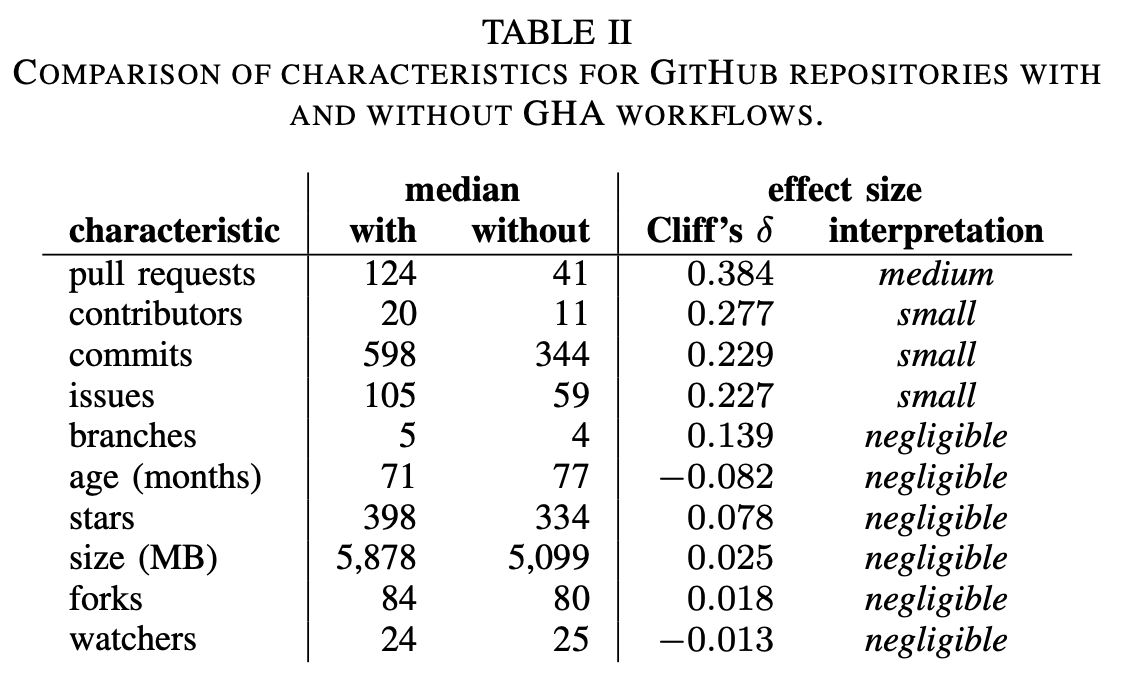
\includegraphics[width=.75\linewidth]{by-metrics.png}
  \source{decan2022use}}

\pitch{Check this repo for inspiration: \href{https://github.com/sdras/awesome-actions}{sdras/awesome-actions} (a curated list of GitHub Action plugins for different purposes).}

\plush{\pptBanner{Some exotic GitHub Action plugins:}
  \begin{itemize}\setlength\itemsep{0em}
  \item \href{https://github.com/hadolint/hadolint-action}{hadolint-action} for \ff{Dockerfile}
  \item \href{https://github.com/marketplace/actions/markdown-lint}{markdownlint-action} for \ff{README.md}
  \item \href{https://github.com/marketplace/actions/shellcheck}{shellcheck-action} for Bash \ff{.sh} scripts
  \item \href{https://github.com/Uno-Takashi/checkmake-action}{checkmake-action} for \ff{Makefile}
  \item \href{https://github.com/ibiqlik/action-yamllint}{action-yamllint} for \ff{YAML} files
  \item \href{https://github.com/yegor256/bibcop-action}{bibcop-action} for Bib\TeX{} \ff{.bib} files
  \end{itemize}}

\end{document}
